\section{Preliminaries}
\label{sec:prelim}

\addin{
Basics definitions and theory for this topic can be found in~\ref{sec:appendix:defs}.

Throughout this paper, a \textbf{\textsf{Theorem}}, \textbf{\textsf{Lemma}}, \textbf{\textsf{Observation}}, or \textbf{\textsf{Remark}} with an asterisk after it means that the proof appears in~\ref{sec:appendix:proofs}.


\subsection{Qusecs}


In this paper, a \dfn{qusecs} is any independent geometric constraint system of one of 3 types: bar-joint (defined formally in \ref{sec:appendix:defs}), \dfn{body-hyperpin} (defined formally in Section \ref{sec:bodypin}), and \dfn{pinned line-incidence} (defined formally in Section \ref{sec:pinnedline}).

% \medskip\noindent
% \note In the remainder of this section and sections~\ref{sec:DRP} and \ref{sec:recomb} we only consider bar-joint qusecs and graphs. Relevant formal analogies for the other 2 types of qusecs and (hyper)graphs are given in the subsequent 2 sections on Applications.

In the remainder of this section and Sections~\ref{sec:DRP} and \ref{sec:recomb} we only consider bar-joint qusecs and graphs. Relevant formal analogies for the other 2 types of qusecs and (hyper)graphs are given in their corresponding sections on applications.
}






\subsection{Decomposition-Recombination (DR) Plans}
%
%$G=(V,E,w_V,w_E)$ is a set of vertices, $V$, and a set of edges, $E$, defined as a tuple of vertices from $V$ (undirected). Additionally, there are two weight functions, $w_V: V \to \mathbb{R}^+$ and $w_E: E \to \mathbb{R}^+$. The \textbf{density} of graph $G$ is $d(G) = \sum_{e\in E}{w_E(e)} - \sum_{v\in V}{w_V(v)}$.
%
%Given a constant $k$, a graph $G$ is:
%\begin{itemize}
%    \item \textbf{independent} (or \textbf{sparse}) if, for all non-trivial subgraphs $S\subseteq G$, $d(S) \leq k$.
%
%    \item \textbf{overconstrained} if it is not independent.
%
%    \item \textbf{wellconstrained} (or \textbf{tight}) if $G$ is independent and $d(G)=k$.
%
%    \item \textbf{rigid} if there exists some spanning subgraph $S\subseteq G$ such that $S$ is wellconstrained.
%
%    \item \textbf{underconstrained} if $G$ is independent and not rigid.
%
%    % \item \textbf{trivial} if (1) it is overconstrained graph and (2) all of its subgraphs are also trivial. Trivial graphs are input.
%\end{itemize}
%
% \begin{definition}
%     A graph is \textbf{overconstrained} if, given constant $k$, there exists some
%     % induced
%     subgraph $S\subseteq G$ such that $d(S) > k$.
% \end{definition}
%
% \begin{definition}
%     A graph is \textbf{wellconstrained} if, given constant $k$, $d(G) = k$ and for all
%     % induced
%     subgraphs $S\subseteq G$, (1) $d(S)\leq k$, or (2) given a set of trivial graphs $T$, $S$ is isomorphic to one of the graphs in $T$ (i.e.\ $S$ is trivial).
% \end{definition}
%
%
%
% \begin{definition}
%     A \textbf{trivial} graph is ill-defined in the general case. The only strict requirements are: (1) it must be an overconstrained graph and (2) all of its subgraphs are also trivial.
%     \todo{Maybe leave the following out until it's needed later?}
%     In the familiar geometric cases of $d$-dimensional space, all vertex weights are $d$, all edge weights are $1$, and constant $k= -{{d+1}\choose{2}}$. Trivial graphs for 2D would be a single vertex. Trivial graphs in 3D would be a vertex and an edge (2 vertices with an edge between). Etc. These trivial graphs capture the notion of the rotational symmetry that exists in geometric spaces.
% \end{definition}
%


\ClearMyMinHeight
\SetMyMinHeight{.4}{img/epsfromtikz/demo_graph}
\SetMyMinHeight{.3}{img/epsfromtikz/demo_graph_comdrp}
\SetMyMinHeight{.3}{img/epsfromtikz/demo_graph_candrp}

\begin{figure*}\centering%
  %
  \begin{subfigure}{0.4\linewidth}\centering
    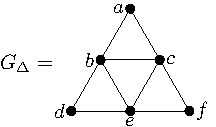
\includegraphics[height=\myMinHeight]{img/epsfromtikz/demo_graph}
    \caption{}\label{fig:demo_graph:graph}
  \end{subfigure}%
  %
  \hfill
  \begin{subfigure}{0.3\linewidth}\centering
    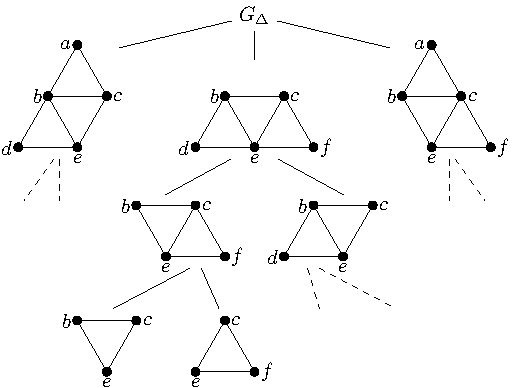
\includegraphics[height=\myMinHeight]{img/epsfromtikz/demo_graph_comdrp}
    \caption{}\label{fig:demo_graph:comdrp}
  \end{subfigure}%
  %
  \hfill
  \begin{subfigure}{0.3\linewidth}\centering
    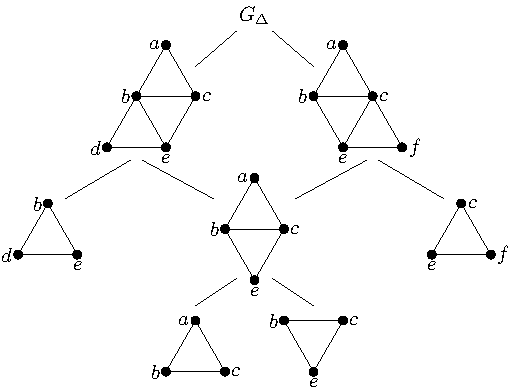
\includegraphics[height=\myMinHeight]{img/epsfromtikz/demo_graph_candrp}
    \caption{}\label{fig:demo_graph:candrp}
  \end{subfigure}%
  %
  \caption{\notetoreviewer{This is a new figure.} \addin{(\ref{fig:demo_graph:graph}) A simple graph, $G_{\Delta}$, used to illustrate concepts throughout this and the next section. (\ref{fig:demo_graph:comdrp}) The complete DR-plan of $G_{\Delta}$, i.e.\ $ComDRP(G_{\Delta})$. Dashed lines indicate that the children repeat the same pattern as the others shown on this level. The children of triangles (3 edges) are omitted. (\ref{fig:demo_graph:candrp}) The canonical DR-plan of $G_{\Delta}$, which is optimal (see Section~\ref{sec:DRP}), i.e.\ $OptDRP(G_{\Delta})$. The children of triangles are omitted.}}
  \label{fig:demo_graph}
\end{figure*}%

\begin{figure*}\centering%
  %
  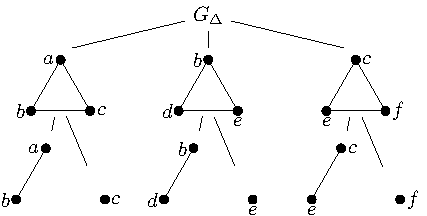
\includegraphics[width=0.4\linewidth]{img/epsfromtikz/demo_graph_clustmindrp}
  \caption{
  \notetoreviewer{This is a new figure.}
  \addin{A DR-plan of $G_{\Delta}$ from Figure~\ref{fig:demo_graph:graph}, which gives cluster minimality. Using the ideas from the paper~\cite{lomonosov2004graph}, the children of a triangle are the primitives of a point and an edge. Thus, the fan-in of this graph is 3, whereas the optimal DR-plans shown in Figure~\ref{fig:demo_graph:candrp} and \ref{fig:demo_graph:candrpseq} have fan-in of 2. With this counterexample, it is clear that cluster minimality is not sufficient for optimality.}
  }
  \label{fig:demo_graph:clustmindrp}
\end{figure*}%


\begin{definition}\label{def:drp}
    The \dfn{decomposition-recombination \mbox{(DR-)} plan} \cite{hoffman2001decompositionI} of graph $G$, $\drp{G}$, \cutout{(see Figure X)} is defined as a forest that has the following properties:
    \begin{enumerate}
        \item Each node represents/contains/is a rigid \cutout{vertex-induced} subgraph of $G$.
        % \item For a node, $C$, that is  a non-trivial graph, its $N$
        % children, $C_1, \ldots, C_N$, are rigid vertex-maximal proper
        % subgraphs of $C$.
        \item Node $C$ has children $C_1,\ldots,C_N$ such that $\bigcup_{i=1}^N{C_i}=C$.
        \item A leaf node is a single vertex. A \dfn{trivial} graph is empty or a single vertex.
        \item A root node is a maximal rigid subgraph of $G$.
    \end{enumerate}
%
    % It can also be described recursively as: the root is $G$, its children are the trivial subgraphs and the DR-plans of its wellconstrained vertex-maximal proper subgraphs whose union is $G$ itself.
%
    A DR-plan is \dfn{complete} if it satisfies an additional rule: for a node $C$ that is  a non-trivial graph, its $N$ children, $C_1, \ldots, C_N$, are all of the rigid vertex-maximal proper subgraphs of $C$. This makes Rule 2 implicit, and in fact, $C$ contains all the edges in the union of its children as well. We denote a complete DR-plan of $G$ as $\comdrp{G}$.

    A DR-plan is \dfn{optimal} if it minimizes the maximum fan-in over all nodes in the tree. The maximum  fan-in is called the \dfn{size} of the DR-plan. We denote an optimal DR-plan of $G$ as $\optdrp{G}$.

    \addin{See Figures \ref{fig:demo_graph}, \ref{fig:c2c3ofk33s}, \ref{fig:demo_graph:candrpseq}, \ref{fig:demo_graph:clustmindrp}, and \ref{fig:bodypindrp} for examples of DR-plans.}

%
%In general, $C$ is the graph in an arbitrary node in $CompleteDRP(G)$.
%$C_i$ is the $i^{\text{th}}$ child of $C$. It is implied that $C_i$ is
%an isostatic vertex-maximal proper subgraph.
    %Note that nodes will be referred to interchangeably as ``the node that
    %represents or contains the (sub)graph $C$'' and as simply ``$C$''.
\end{definition}
%
% \todo{This was labeled as both begin(remark) and end(observation), what was your intent?}
\begin{remark}
    For a given graph, there could be exponentially many  DR-plans and even optimal DR-plans in the size of the graph. A complete DR-plan is unique but may not be (is usually not) optimal. DR-plans of self-similar graphs are self-similar. More than one node (leaf) in a DR-plan forest may represent the same subgraph (vertex) of $G$.
\end{remark}

\cutout{
\noindent
\textbf{Note:} In Section X, $G$ is assumed to be isostatic.
}

% \begin{definition}
%     The \textbf{complete DR-plan} of graph $G$, $CompleteDRP(G)$, is the unique DR-plan but with a modified rule number 2: the children are \emph{all} of the trivial or wellconstrained vertex-maximal proper subgraphs of that node $C$. By this, rule 3 is implicit for a complete DR-plan.
% \end{definition}

% \begin{definition}
%     The \textbf{optimal DR-plan} of graph $G$, $OptimalDRP(G)$, is the DR-plan that minimizes the maximum fan-in over all nodes in the tree. It is not necessarily unique.
% \end{definition}




%\emph{wellconstrained} bar and joint graph with values $(V,E,w_V,w_E)$.
% \todo{I don't think the following is actually necessary to mention...} To keep problems meaningful we assume that $G$ is connected, as the methods discussed are used to solve systems of equations to establish linkages. It is not useful to solve for two bodies simultaneously if there are no constraints between them.
% THIS MEANS NO EDGES MAY BE LEFT OUT, ALSO.


\subsection{Importance of an Optimal DR-plan}
The use of a DR-plan in designing especially self-similar qusecs is immediately evident, shown in Figures \ref{fig:c2c3ofk33s} and \ref{fig:bodypindrp}.

In fact, knowing an optimal DR-plan is crucial for design and analysis of even non-self-similar qusecs and their realizations with various desirable properties.

\medskip\noindent
\header{Realizing given qusecs.}
Note that this basic task would require finding real solutions \addin{to} a large multivariate polynomial system (of inequalities and equalities representing the constraints). Without DR-planning, this requires double exponential time in the number of variables (even if orientation type is specified). With DR-planning, the complexity is dominated by the size of the largest subsystem that is solved, or recombined from the solutions of its child subsystems\addin{,} i.e., the maximum fan-in occurring in a DR-plan. Thus\addin{,} finding an optimal DR-plan is important for realization.

\medskip\noindent
\header{Recursive block decomposition of the rigidity matrix, stress space and external stresses.}
This can be obtained using the DR-plan\addin{,} \cutout{we obtain a} with each block being the rigidity matrix of an isostatic subgraph. The blocks intersect on isostatic or trivial subgraphs. This recursive block decomposition of the rigidity matrix $R$ correspondingly recursively decomposes the stress vectors $s$ that balance a given external stress $t$ since $sR = t$. Moreover, the external stress vector $t$ is recursively ``distributed'' into external stresses for each node of the DR-plan. When the rigidity matrix and stress vectors contain indeterminates, this  can be used to design underlying graph and parameters $\delta$ to obtain an optimal distribution of stresses on the geometric primitives. When the realization of qusecs is given, this can be used to analyze the distribution of a given external load.




%\subsection{DR-plan}
%%\subsection{Definitions}
%%\label{sec:prelim_defs}
%%
%%% TODO
%%
%%% A paragraph of preliminaries such as:
%%%     - rigidity matrix R,
%%%     - stress vectors S one coordinate per edge (w/ SR =E (external stress vector, 2 coordinates  per vertex));
%%%     - flex vectors F (2 coordinates per vertex) (right nullspace/kernel of R)
%%% Should precede the definition of
%%%     + independent,
%%%     + overconstrained (not independent),
%%%     - rigid (contains an independent set with sufficiently many eedges/constraints)
%%%     - isostatic (wellconstrained/minimally rigid), ,
%%%     - flexible (not rigid),
%%%     + underconstrained (independent and not rigid).
%%% After that, define DR plans etc.
%%
%%In Sections \ref{sec:DRP} and \ref{sec:recomb} a \textbf{graph} is a bar and joint system. $G=(V,E,w_V,w_E)$ is a set of vertices, $V$, and a set of edges, $E$, defined as a tuple of vertices from $V$ (undirected). Additionally, there are two weight functions, $w_V: V \to \mathbb{R}^+$ and $w_E: E \to \mathbb{R}^+$. The \textbf{density} of graph $G$ is $d(G) = \sum_{e\in E}{w_E(e)} - \sum_{v\in V}{w_V(v)}$.
%%
%%Given a constant $k$, a graph $G$ is:
%%\begin{itemize}
%%    \item \textbf{independent} (or \textbf{sparse}) if, for all non-trivial subgraphs $S\subseteq G$, $d(S) \leq k$.
%%
%%    \item \textbf{overconstrained} if it is not independent.
%%
%%    \item \textbf{wellconstrained} (or \textbf{tight}) if $G$ is independent and $d(G)=k$.
%%
%%    \item \textbf{rigid} if there exists some spanning subgraph $S\subseteq G$ such that $S$ is wellconstrained.
%%
%%    \item \textbf{underconstrained} if $G$ is independent and not rigid.
%%
%%    % \item \textbf{trivial} if (1) it is overconstrained graph and (2) all of its subgraphs are also trivial. Trivial graphs are input.
%%\end{itemize}
%%
%\textbf{Trivial} graphs are ill-defined in the general case. The only strict requirements are: (1) it must overconstrained and (2) all of its subgraphs are also trivial.
%
%% \begin{definition}
%%     A graph is \textbf{overconstrained} if, given constant $k$, there exists some
%%     % induced
%%     subgraph $S\subseteq G$ such that $d(S) > k$.
%% \end{definition}
%
%% \begin{definition}
%%     A graph is \textbf{wellconstrained} if, given constant $k$, $d(G) = k$ and for all
%%     % induced
%%     subgraphs $S\subseteq G$, (1) $d(S)\leq k$, or (2) given a set of trivial graphs $T$, $S$ is isomorphic to one of the graphs in $T$ (i.e.\ $S$ is trivial).
%% \end{definition}
%
%
%
%% \begin{definition}
%%     A \textbf{trivial} graph is ill-defined in the general case. The only strict requirements are: (1) it must be an overconstrained graph and (2) all of its subgraphs are also trivial.
%%     \todo{Maybe leave the following out until it's needed later?}
%%     In the familiar geometric cases of $d$-dimensional space, all vertex weights are $d$, all edge weights are $1$, and constant $k= -{{d+1}\choose{2}}$. Trivial graphs for 2D would be a single vertex. Trivial graphs in 3D would be a vertex and an edge (2 vertices with an edge between). Etc. These trivial graphs capture the notion of the rotational symmetry that exists in geometric spaces.
%% \end{definition}
%
%
%\begin{definition}\label{def:drp}
%    The \textbf{decomposition-recombination \mbox{(DR-)} plan} of graph $G$, $DRP(G)$, is defined as a tree that has the following properties:
%    \begin{enumerate}
%        \item The root of the tree `contains' $G$.
%        \item For all nodes, $C$, that `contain' non-trivial graphs, its $N$ children, $C_1, \ldots, C_N$, are trivial or wellconstrained vertex-maximal proper subgraphs of that node $C$.
%        \item The vertex set of $\bigcup_{i=1}^N{C_i}$ is the vertex set of $C$.
%        \item A node with a trivial subgraph is a leaf.
%    \end{enumerate}
%
%    % It can also be described recursively as: the root is $G$, its children are the trivial subgraphs and the DR-plans of its wellconstrained vertex-maximal proper subgraphs whose union is $G$ itself.
%
%    An equivalent DAG can be constructed from this tree such that all nodes containing the same subgraphs are combined into one, with all edges preserved.
%
%    Note that nodes will be referred to interchangeably as ``the node that contains the (sub)graph $C$'' and as simply ``$C$''.
%
%    A DR-plan is \textbf{complete} if it satisfies the modified rule number 2: the children are \emph{all} of the trivial or wellconstrained vertex-maximal proper subgraphs of that node $C$. This makes rule 3 implicit. The complete DR-plan is unique.
%
%    A DR-plan is \textbf{optimal} if it minimizes the maximum fan-in over all nodes in the tree. It is not necessarily unique.
%\end{definition}
%
%% \begin{definition}
%%     The \textbf{complete DR-plan} of graph $G$, $CompleteDRP(G)$, is the unique DR-plan but with a modified rule number 2: the children are \emph{all} of the trivial or wellconstrained vertex-maximal proper subgraphs of that node $C$. By this, rule 3 is implicit for a complete DR-plan.
%% \end{definition}
%
%% \begin{definition}
%%     The \textbf{optimal DR-plan} of graph $G$, $OptimalDRP(G)$, is the DR-plan that minimizes the maximum fan-in over all nodes in the tree. It is not necessarily unique.
%% \end{definition}
%
%
%\subsection{Notation}
%
%In Sections \ref{sec:DRP} and \ref{sec:recomb}, $G$ is taken to be a \emph{wellconstrained} bar and joint graph with values $(V,E,w_V,w_E)$.
%% \todo{I don't think the following is actually necessary to mention...} To keep problems meaningful we assume that $G$ is connected, as the methods discussed are used to solve systems of equations to establish linkages. It is not useful to solve for two bodies simultaneously if there are no constraints between them.
%% THIS MEANS NO EDGES MAY BE LEFT OUT, ALSO.
%
%$Idc(G,X)$ is the graph induced on $G$ with the vertex set $X\subseteq V$. This can also be overloaded such that, using graph $H=(W,F)$, $Idc(G,H)=Idc(G,W)$.
%
%$C$ is the graph in an arbitrary node in $CompleteDRP(G)$. $C_i$ is the $i^{\text{th}}$ child of $C$. By definition of a DR-plan, it is implied that $C_i$ is a wellconstrained vertex-maximal proper subgraph.
